% Dyna-Bound manuscript for The Journal of Supercomputing
% Build: bash build.sh
\documentclass[11pt,a4paper]{article}

\usepackage[margin=2.5cm]{geometry}
\usepackage{times}
\usepackage{amsmath,amssymb,amsfonts}
\usepackage{graphicx}
\usepackage{booktabs}
\usepackage{xcolor}
\usepackage{hyperref}
\usepackage{url}
\usepackage{natbib}
\usepackage{algorithm}
\usepackage{algpseudocode}
\usepackage{setspace}
\usepackage{caption}
\usepackage{placeins}
\hypersetup{colorlinks=true,linkcolor=black,citecolor=blue,urlcolor=blue}
\graphicspath{{figures/}}
\setstretch{1.05}
\captionsetup{font=small,labelfont=bf}

\title{Colony-Bounded Hybrid Learning for Cold-Start Fog Service Placement}

\author{
Rouhollah Nabati$^{1}$\thanks{Corresponding author: Rouhollah Nabati.}\\
Abdulbaghi Ghaderzadeh$^{1}$\\[0.6em]
\small $^{1}$Department of Computer Engineering, Faculty of Engineering,\\
\small Islamic Azad University, Sanandaj Branch, Sanandaj, Iran
}

\date{}

\begin{document}
\maketitle

%% --- Springer Nature sn-jnl swap (when cls is available) ---
%% \documentclass[pdflatex,sn-mathphys-ay]{sn-jnl}
%% \begin{abstract}
When fog nodes arrive under burst load and membership change, a placement
policy that assumes a ready hierarchy or a near-global host list either spends
heavily on control traffic or fails early. We study the complementary problem:
learning to rank hosts \emph{inside} an already bounded cold-start control plane.
\textbf{Dyna-Bound} keeps DynaCol colony formation, FCM handover, and CRT/GRT
tables unchanged, and replaces only local L2 ranking. An online scorer---a small
GraphSAGE encoder or a flat vector---is mixed with the deterministic DCBO
objective and is switched off once the fabric is large enough for exact DCBO.
On iFogSim2 multipipe workloads ($N{=}100$, 20 paired trials) both hybrids cut
mean SLA violation relative to DCBO at matched CRT/GRT overhead; paired gaps
remain significant after Holm correction (Cohen's $d$ roughly $0.6$--$1.1$).
The two encoders are statistically tied, so the result is about bounded hybrid
ranking, not a general GNN advantage. Ablations show that widening the action
set beyond CRT improves absolute SLA at the price of the visibility the colony
tables withhold; at $N{=}1000$ the methods converge under the large-scale gate.
\end{abstract}
%% Required declarations (also kept below for article-class builds):
%% \bmhead{Acknowledgements} ...
%% Competing interests / Funding / Data availability / Author contributions

\begin{abstract}
Fog service placement is hard when the control plane must form from scratch
under burst load and membership churn. Many learning placers assume an
organized hierarchy or a near-global host set, so control cost and cold start
are rarely isolated. We present \textbf{Dyna-Bound}, a colony-bounded hybrid
that reuses DynaCol cold-start formation and bounded neighbor tables, changing
only local ranking: online GraphSAGE or flat-vector scores mix with a
deterministic colony objective and return to it at large scale. In iFogSim2, a
20-trial multipipe study shows both hybrids reduce mean SLA violation versus
that baseline at matched control overhead, with Holm-significant paired gaps
(Cohen's $d$ about $0.6$--$1.1$). GraphSAGE and the vector ablation are
statistically tied; a same-plane tabular learner is an SLA control, not the
claim. Ablations show the colony bound trades absolute SLA for decentralized
visibility; methods stay close at one thousand fog nodes.
\end{abstract}

\noindent\textbf{Keywords:}
fog computing, service placement, hybrid learning, cold start,
self-organizing systems, graph neural networks, CRT/GRT, iFogSim2

\section{Introduction}
\label{sec:intro}

Fog and edge placement must keep end-to-end delay inside SLA limits while demand,
membership, and link quality change
\cite{bonomi_mcc2012,chiang_jiot2016,yousefpour_sysarc2019,mouradian_comst2018}.
Under burst arrivals and node departures, controllers that wait for a global
snapshot, or that assume a finished hierarchy, either flood the network with
control messages or miss early requests
\cite{salaht_csur2020,taleb_csur2025_survey,gasmi_jsup2021_survey}.
Learning-based placers adapt under shifting load
\cite{supraja_cluster2025_slr,schulman_ppo2017,haddadha_aire2024_mlplacement},
but many still treat almost every host as a legal action and rarely account for
the messaging cost of that choice
\cite{hong_csur2019_resource,abdulazeez_access2023_offload}.

Our prior control plane, DynaCol, already forms colonies from an empty state,
elects and hands over an FCM, and keeps CRT/GRT neighbor tables bounded. DCBO is
its default L2 scorer, with sticky L1 reuse and cloud L3 fallback. What it does
not provide is an online learner that is \emph{required} to choose inside those
same tables. That constraint is the focus of this paper: if the control plane
must stay cheap and decentralized, can hybrid learning still improve SLA without
opening a near-global host set?

Dyna-Bound leaves formation, handover, CRT/GRT, L1, and L3 as in DynaCol and
changes only L2 ranking (Fig.~\ref{fig:arch}). A small online scorer is added to
the inverted DCBO utility; the learning weight falls with fog count and is set
to zero beyond a live-node gate so large fabrics return to exact DCBO. We try
two scorers with the same hybrid rule: a HID$=$16 GraphSAGE encoder on RTT
affinity and service-DAG context (with optional offline import and fine-tune),
and a flat vector without message passing (Fig.~\ref{fig:encoders}). GraphSAGE is
the structured default; it is not offered as proof that GNNs always beat linear
scores on CRT neighborhoods.

After cold start the action set satisfies $|A_t|\le K_{\mathrm{crt}}$, so the
overlay is part of the learning problem rather than an external assumption.
We evaluate on iFogSim2 under normal, burst, and churn loads against DCBO at
matched CRT/GRT overhead, with a tabular $\varepsilon$-greedy learner and
lightweight CRT-bounded DQN/PPO variants as additional colony-plane references,
plus named flat baselines for absolute SLA context. The primary statistical
evidence is a 20-trial multipipe grid with paired tests, Holm adjustment,
bootstrap intervals, and Cohen's $d$, supported by sensitivity checks, an
$N{=}1000$ run, CRT/offline/$\beta$ ablations, and a separate node-failure stress
test.

\paragraph{Contributions.}
\begin{enumerate}
\item A colony-bounded MDP in which feasible L2 actions are the CRT top-$K$
(and limited GRT escalation), so cold-start visibility is a hard learning
constraint rather than a soft preference.
\item A hybrid L2 rule that mixes an online score with DCBO and hands ranking
back to exact DCBO at large scale; the main empirical claim is Hybrid $\succ$
DCBO at matched control overhead on the multipipe journal grid.
\item Two interchangeable scorers under that rule (GraphSAGE and vector) plus
colony-plane reference learners (tabular $\varepsilon$-greedy, lightweight
DQN/PPO), used to separate the hybrid design from any single encoder story.
\item An empirical package on iFogSim2: $n{=}20$ multipipe tests with effect
sizes, scale and sensitivity checks, CRT visibility ablations, flat-baseline
Pareto context, and hard router-failure trials at $5$--$20\%$.
\end{enumerate}

\section{Related Work}
\label{sec:rw}

\subsection{Fog and edge service placement}
Fog computing extends the cloud toward latency-sensitive, geo-distributed IoT
workloads \cite{bonomi_mcc2012,chiang_jiot2016,mouradian_comst2018,naha_access2018_fog}.
Surveys of service placement and offloading catalogue latency, energy, and cost
objectives under fixed or centralized controllers
\cite{salaht_csur2020,smolka_computing2022_eval,gasmi_jsup2021_survey,taleb_csur2025_survey,apat_computers2025_survey,yousefpour_sysarc2019}.
Classical and heuristic mappers assign modules along fog--cloud paths
(Edgeward-style resource-aware placement, FogTorch / FogTorch$\Pi$ QoS matching,
optimized IoT placement, and FogPlan Min-Cost)
\cite{taneja_im2017_edgeward,brogi_jiot2017_fogtorch,brogi_icfec2017_fogtorchpi,skarlat_icfec2017,skarlat_soca2017,yousefpour_fogplan_jiot2019}.
Metaheuristics and ILP-style workload allocation further improve mapping quality
once a topology is given
\cite{azimzadeh_cluster2022_genetic,benamer_cluster2024_ga,deng_jiot2016_workload,guerrero_fgcs2019_evolutionary}.
These lines assume an already organized fabric or a global/central view; they do
not form a self-organizing overlay from an empty colony state, nor do they treat
a bounded neighbor table as a hard action set for online learning.

\subsection{Learning-based offloading and placement}
DQN/PPO-style and broader ML placers adapt under changing demand
\cite{mnih_nature2015_dqn,schulman_ppo2017,supraja_cluster2025_slr,haddadha_aire2024_mlplacement,abdulazeez_access2023_offload}.
Recent DRL work targets healthcare/fog stacks, energy-aware modules, multi-tier
containers, microservice instance selection, and IoT job deployment
\cite{tuli_iotj2020_dynamic,hossam_cluster2024_energy,dogani_cluster2024_twotier,boudieb_fgcs2024_drl,bushehrian_computing2025_drl}.
Resource-management and orchestration surveys still note large action spaces and
the assumption of an organized fabric
\cite{hong_csur2019_resource,costa_csur2022,pallewatta_csur2023_microservices,mahmud_csur2020_appmgmt}.
Dyna-Bound keeps $|A_t|$ inside CRT/GRT top-$K$, mixes learning with DCBO, and
reports the same table overhead as the colony control plane. The point is not
another open-set DRL placer, but a learner that cannot leave the cold-start
view.

\subsection{Self-organizing and hierarchical fog control}
Overlay formation, manager election, and hierarchical module managers separate
structure from placement
\cite{mahmud_fog_application2018,bittencourt_cloudcomp2017_mobility,ouyang_jiot2021_drloffload}.
Evolutionary and mobility-aware schedulers improve QoS once a hierarchy exists
\cite{guerrero_fgcs2019_evolutionary}, but learning is seldom constrained to the
colony view as a hard limit. Here formation and FCM handover stay with DynaCol;
learning only re-ranks inside that view.

\subsection{Graph learning on infrastructure and service graphs}
Message-passing encoders (GCN, GraphSAGE, GIN, GAT) provide inductive structure
models for neighborhoods and dependency graphs
\cite{kipf_gcn_iclr2017,hamilton_graphsage2017,xu_gin_iclr2019,velickovic_gat2018}.
GNN-RL placers encode service and/or MEC graphs for multi-objective mapping and
adaptive microservice placement, including dual-GNN DDPG designs
\cite{lera_jsup2024_gnn,chen_tmc2024_dgddpg}.
Those peers typically optimize over broader device sets than a cold-start CRT.
Our CRT neighborhoods are small and RTT-structured, so local message passing is
cheap if the action set stays colony-bounded. On the multipipe journal grid the
GraphSAGE and vector scorers land statistically together; the hybrid rule, not
the encoder family, is what we defend against DCBO.

\subsection{Relation to DynaCol}
DynaCol/DCBO is the prior control plane and the matched-overhead baseline
\cite{nabati_dynacol_cluster2026}. Cold-start formation and FCM handover are
not restated as new results. The companion DynaCol write-up is cited as an
unpublished control-plane artifact; the reused algorithms are reprinted in
Appendix~\ref{app:dynacol} so this paper stays readable on its own. What is new
here is the colony-bounded L2 MDP, the hybrid GraphSAGE/vector ranking with a
scale-aware blend, the colony-plane reference learners, and the multipipe
evaluation package.

\begin{table}[t]
\centering
\caption{Where Dyna-Bound sits relative to common placement families.}
\label{tab:positioning}
\scriptsize
\setlength{\tabcolsep}{3pt}
\resizebox{\columnwidth}{!}{%
\begin{tabular}{@{}lcccc@{}}
\toprule
Method family & Cold-start & Bounded view & Hybrid w/ determ.\ obj. & Local graph/DAG \\
\midrule
Classical / GA / ILP & Rarely & No & Sometimes & Rarely \\
FogPlan / Edgeward / Static-DCBO & No/partial & No/fixed & No & No \\
DRL placers (DQN/PPO) & Rarely & Rarely & Rarely & Sometimes \\
GNN-RL placers & Rarely & Rarely & Rarely & Yes \\
DynaCol / DCBO & Yes & Yes & N/A & No \\
\textbf{Dyna-Bound} & \textbf{Yes} & \textbf{Yes} & \textbf{Yes} & \textbf{Yes} \\
\bottomrule
\end{tabular}%
}
\end{table}

We use iFogSim / iFogSim2 for simulation
\cite{gupta_ifogsim2017,mahmud_ifogsim2_jss2022}
(EdgeCloudSim is a related alternative \cite{sonmez_edgecloudsim2018})
and Holm's procedure for multiple comparisons \cite{holm_1979}, with Cohen's
$d$ for paired effect sizes \cite{cohen_power1988}.

\section{Background: DynaCol Control Plane}
\label{sec:bg}

Only the reused pieces are summarized here
\cite{nabati_dynacol_cluster2026}; pseudocode appears in
Appendix~\ref{app:dynacol}.

Nodes join by query/advertise until colonies appear. An FCM is elected by
potency and updated with $\varepsilon$-greedy probes and a cooldown on handover.
Each FCM keeps a CRT of member capacity, availability, RTT, and attractiveness
(default top-$K_{\mathrm{crt}}{=}5$); GRT summaries allow limited cross-colony
search (default top-$K_{\mathrm{grt}}{=}3$) without a full host list.
Placement is three-tier: sticky L1 reuse if the current host still meets SLA
thresholds; DCBO L2 scoring over CRT then GRT; cloud L3 if both fail.
Dyna-Bound replaces only the L2 ranking inside CRT/GRT top-$K$
(Fig.~\ref{fig:arch}).

\begin{figure}[htbp]
\centering
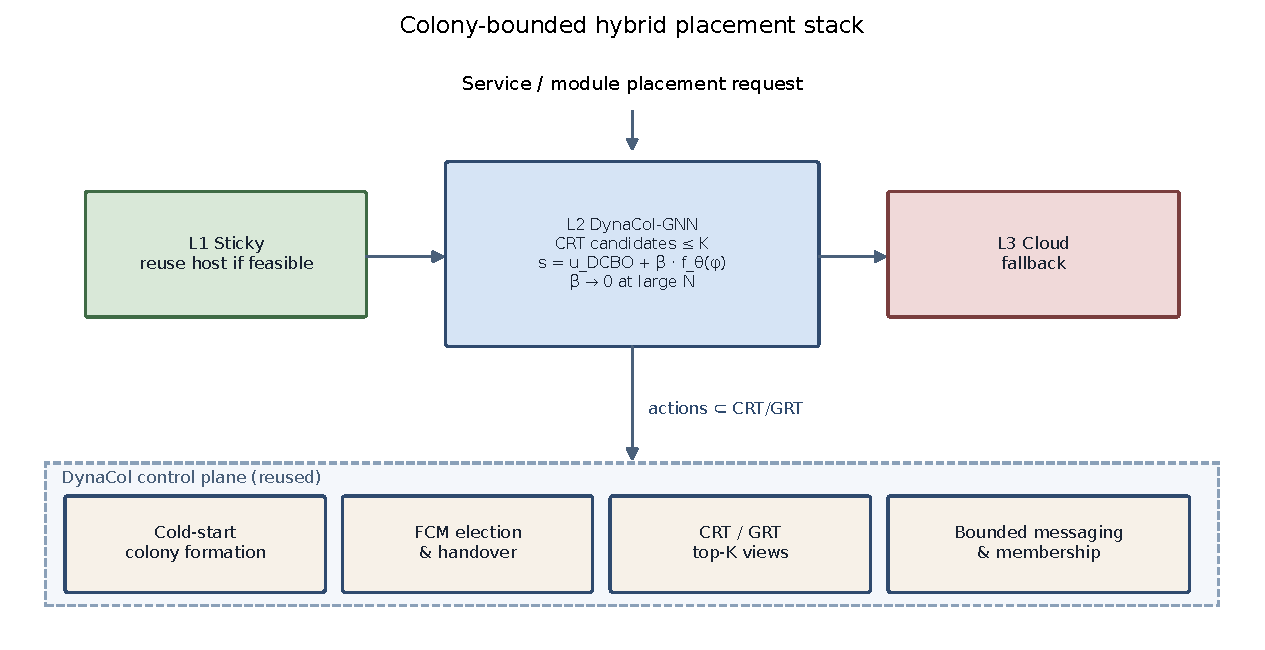
\includegraphics[width=\linewidth]{fig01_architecture.pdf}
\caption{Placement stack on the reused DynaCol control plane: L1 sticky reuse,
L2 Dyna-Bound over CRT/GRT, L3 cloud fallback.}
\label{fig:arch}
\end{figure}

\section{Colony-Bounded Hybrid Learning}
\label{sec:method}

\subsection{MDP}
On each FCM reconcile, state $S_t$ is the local CRT (size $\le K_{\mathrm{crt}}$),
optional GRT summaries, and service/DAG features. Action $A_t$ picks a feasible
CRT host or escalates to GRT/L3. The hard limit $|A_t|\le K_{\mathrm{crt}}$ is
intentional: the control plane is part of the learning method.

Host features (dimension 8) and service/context features (dimension 8) are
listed in Table~\ref{tab:features}. Continuous resource channels are scaled by
the colony-local maximum available value; RTT is clipped by $100$\,ms; deadline
context is clipped by $500$\,ms. No learned feature weights are applied before
the encoder; the vector ablation zeros DAG topology and co-location channels so
message passing remains the main encoder difference.

\begin{table}[htbp]
\centering
\caption{Candidate features used online (no PCA or other dimensionality reduction).}
\label{tab:features}
\small
\begin{tabular}{@{}llp{0.42\linewidth}@{}}
\toprule
Group & Feature & Normalization / note \\
\midrule
Host & CPU, RAM, storage, BW & available / colony max \\
Host & RTT to FCM & $\min(1,\mathrm{RTT}/100)$ \\
Host & Attractiveness & clipped to $[-1,1]$ \\
Host & Neighbor pressure, edge entropy & GraphSAGE only; else $0$ \\
Context & Demand CPU/RAM & demand / colony max \\
Context & Deadline & $\min(1,D/500)$ \\
Context & In/out degree, depth, source/sink & DAG norms (GraphSAGE); Vector zeros \\
Context & Producer-RTT pull, fan-in, co-location & GraphSAGE; Vector zeros co-location \\
\bottomrule
\end{tabular}
\end{table}

\paragraph{Reward.}
Let $r_{\mathrm{attr}}$ be the attractiveness reward used by DCBO and
$r_{\mathrm{dcbo}}$ the same signal at the DCBO-preferred CRT host. The shaped
online target is
\begin{equation}
R_t=\mathrm{clip}_{[0,1]}\bigl(0.5+0.5(r_{\mathrm{attr}}-r_{\mathrm{dcbo}})\bigr).
\end{equation}
For GraphSAGE, a graph-SLA score (producer-RTT pull, co-location under fan-in) further
biases the contrastive update. Vector uses the same $R_t$ with a weak linear
TD-style update on the chosen feature vector.

\subsection{Hybrid scoring}
\begin{equation}
s(i)=u_{\mathrm{DCBO}}(i)+\beta\cdot f_\theta\bigl(\phi(i)\bigr),
\label{eq:hybrid}
\end{equation}
with $u_{\mathrm{DCBO}}$ the inverted DCBO objective. We take $\arg\max_i s(i)$
and allow a small $\varepsilon$-greedy rate while $n_f$ is below the large-scale
gate. The blend $\beta$ falls with fog count (default $0.60$ on multipipe at
small $N$) and is set to zero for $n_f\ge 450$, so L2 becomes exact DCBO.

\subsection{Encoders}
The vector policy (\texttt{colony\_rl}) concatenates host channels with
service/DAG scalars and scores with a linear head (learning rate $0.05$). The
GraphSAGE policy (\texttt{colony\_gnn}) builds a structure-aware affinity graph on CRT
candidates: RTT base \(A_{ij}\propto 1/(1+\mathrm{RTT}_{ij}/20)\) plus coloc and
producer-host pull (RTT-only ablation via a system flag), then a two-layer
GraphSAGE-style update (hidden width $16$)
\begin{equation}
h'=\tanh\bigl(W_{\mathrm{self}}h+W_{\mathrm{neigh}}Ah\bigr),
\end{equation}
then reads out from $\mathrm{concat}(h,\mathrm{context})$ (learning rate
$0.04$). Offline JSON weights can be loaded and fine-tuned online
(Fig.~\ref{fig:encoders}).

A tabular $\varepsilon$-greedy baseline (\texttt{drl}) keeps cold-start CRT/GRT
formation but replaces L2 with attractiveness selection
($\varepsilon{=}0.15$), without a neural encoder or DCBO hybridization. We also
include two lightweight CRT-bounded neural references (\texttt{colony\_dqn},
\texttt{colony\_ppo}): shared one-hidden-layer scorers on the same flat features
as the vector path, with a one-step TD update (DQN-style) or a clipped
likelihood-ratio nudge with a moving baseline (PPO-style). They are not full
open-set deep RL stacks; they only ask whether a small neural ranker inside
CRT can match the hybrid under the same action bound.

\begin{figure}[htbp]
\centering

\includegraphics[width=\linewidth]{fig02_encoders.pdf}
\caption{Dyna-Bound Vector and GraphSAGE encoder pipelines into the same hybrid score
\eqref{eq:hybrid}.}
\label{fig:encoders}
\end{figure}

\subsection{Online updates and offline import}
After $i^\star$ is chosen, GraphSAGE applies a centered advantage update
$R_t-\bar R$ with a soft contrastive push toward the graph-SLA-best CRT index
when available; Vector applies a delta rule on the chosen features toward
$R_t$. Attractiveness decay/update mirrors DCBO.

\paragraph{Offline path.}
Exploratory \texttt{colony\_gnn} runs log CRT tensors (host matrix, context,
adjacency, action, reward, optional DCBO base scores). Outside the simulator we
train a GIN-style encoder \cite{xu_gin_iclr2019} matching the Java layout with
\textbf{reward-advantage behavioral cloning plus structure ranking} (not classic
PPO), in the spirit of imitation / offline policy learning from logged
trajectories \cite{ross_aistats2011_dagger,levine_offline_rl2020}: weighted NLL on the logged action, softplus ranking between
structure-best/worst hosts, an optional ranking term against the inverted DCBO
base vector, and a small entropy bonus. Exported JSON tensors load into the
online GraphSAGE; champion and journal grids enable online fine-tuning.

\subsection{Complexity}
\label{sec:complexity}
Let $K{=}K_{\mathrm{crt}}$ (default $5$), host/context width $d{=}8$, and GraphSAGE
hidden width $h{=}16$. Per reconcile after cold start:
\begin{itemize}
\item \textbf{Query.} Read at most $K$ CRT rows and optional $K_{\mathrm{grt}}$ GRT
summaries: $O(K+K_{\mathrm{grt}})$.
\item \textbf{Scoring.} Feature build is $O(Kd)$. Vector scoring is $O(Kd)$.
GraphSAGE with dense CRT affinity is $O(K^2 d+K h(d+h))$ and stays constant-order
for fixed $K,h$. Hybrid blend with DCBO utility is $O(K)$.
\item \textbf{Update.} Vector delta rule $O(d)$; GraphSAGE centered advantage on
the chosen neighborhood $O(K h(d+h))$.
\end{itemize}
Total decision time is therefore $O(K)$ in the CRT size with fixed $d,h$, not
$O(N)$ in the fog population. Memory is $O(K)$ for CRT, $O(K_{\mathrm{grt}})$ for
GRT, plus $O(dh+h^2)$ encoder weights (HID$=$16). Offline GIN training is done
outside the control loop; online fine-tune uses the same small parameter set.
Control messaging remains the CRT/GRT traffic of DynaCol.

\begin{algorithm}[t]
\caption{Colony-bounded hybrid reconcile (sketch)}
\label{alg:reconcile}
\begin{algorithmic}[1]
\Procedure{Reconcile}{$r$, fcm, current}
  \If{$\beta\approx 0$}
    \State \Return DCBO.reconcile($\ldots$)
  \EndIf
  \If{L1 sticky OK}
    \State \Return current
  \EndIf
  \If{CRT enabled}
    \State $C\leftarrow$ top-$K$ feasible CRT entries
    \State pick $i^\star$ by hybrid score on $\phi(C)$; update $\theta$
    \State \Return host($i^\star$)
  \EndIf
  \If{GRT enabled}
    \State escalate via ranked GRT summaries
  \EndIf
  \State \Return cloud \Comment{L3}
\EndProcedure
\end{algorithmic}
\end{algorithm}

\section{Experimental Setup}
\label{sec:setup}

Simulations run in iFogSim2 on the shared DynaCol runtime
\cite{gupta_ifogsim2017,mahmud_ifogsim2_jss2022}.
We compare \texttt{dcbo}, \texttt{colony\_rl} (Vector),
\texttt{colony\_gnn} (GraphSAGE), tabular \texttt{drl}, and the lightweight
CRT-bounded \texttt{colony\_dqn}/\texttt{colony\_ppo} scorers above, plus flat
\texttt{static\_dcbo}, \texttt{fogplan} \cite{yousefpour_fogplan_jiot2019}, and
\texttt{greedy}. Edgeward-style module mapping
\cite{taneja_im2017_edgeward} was dropped on multipipe after single trials
exceeded 25 minutes. The DQN/PPO variants never expand the action set beyond
CRT top-$K$; they are colony-plane references, not re-implementations of
open-host DQN/PPO placers from the broader literature.

\subsection{Topology and workload}
The fabric is a four-tier iFogSim hierarchy: one cloud, a proxy, fog routers, and
camera leaves. Fog routers use about $2800$--$5600$\,MIPS and $4$\,GB RAM; cameras
about $500$\,MIPS and $1$\,GB RAM; uplink/downlink bandwidth on fog links is
$10$\,Gbps-class in the simulator defaults. Target sizes are
$N\in\{100,300,500,1000\}$ under normal, burst, and churn. We also inject hard
fog-router failures at mid-run for fractions $5\%$, $10\%$, and $20\%$ of
router nodes (\texttt{node\_fail05/10/20}), reporting SLA\% after failure plus
hosts failed, modules displaced, and approximate recovery time to the first
post-failure reconcile. The surveillance DAG
is the shallow camera pipeline; the multipipe DAG adds fan-out, skip, and join
edges (Fig.~\ref{fig:dag}).

\subsection{SLA violation metric}
\label{sec:sla}
Let $L_j$ be the end-to-end loop delay (ms) of completed request $j$, and let
$M$ be the number of completed loop samples in a trial. The deadline (ms) is
\begin{equation}
D(N,s,\sigma)=\sigma\cdot\alpha(s)\bigl(60+N/10\bigr),
\label{eq:deadline}
\end{equation}
where $\alpha(\mathrm{normal}){=}1$, $\alpha(\mathrm{burst}){=}0.85$,
$\alpha(\mathrm{churn}){=}0.88$, and $\sigma$ is the deadline scale
($\sigma{=}10$ on the locked multipipe grids; $\sigma{=}1$ on surveillance unless
noted). Request $j$ violates the SLA if $L_j>D$; the reported violation rate is
\begin{equation}
\mathrm{SLA\%}=100\cdot\frac{1}{M}\sum_{j=1}^{M}\mathbf{1}[L_j>D].
\label{eq:slaviol}
\end{equation}
Sensor periods are $5$\,ms (normal/churn) and $1$\,ms (burst). We also report
P95 loop delay, normalized control overhead, and colony count.

\subsection{Statistics}
The tuning lock uses 5 trials; the journal $N{=}100$ multipipe grid uses
\textbf{20} paired trials. For each method pair we report mean $\pm$ std of
SLA\%, a paired $t$-test, Holm-adjusted $p$-values across the comparison family
\cite{holm_1979}, percentile bootstrap 95\% CIs on the paired mean difference,
and Cohen's $d$ on paired differences \cite{cohen_power1988}. $N{=}1000$ uses
10 trials; flat baselines use 5 trials. One-factor sensitivity sweeps
($\beta$, deadline scale, $\varepsilon$) use 5 Burst trials. Locked settings:
HID$=$16, $\beta{=}0.60$, $\varepsilon{=}0.02$, offline weights with fine-tune.
Companion 5-trial ablations isolate the CRT action bound, offline import, and
$\beta{=}0$ DCBO delegation (Sec.~\ref{sec:ablations}).

\begin{figure}[htbp]
\centering

\includegraphics[width=0.95\linewidth]{fig03_multipipe_dag.pdf}
\caption{Multipipe application DAG used in the champion and journal grids.}
\label{fig:dag}
\end{figure}
\FloatBarrier

\section{Results}
\label{sec:results}

\subsection{Journal multipipe grid ($n{=}20$)}
Table~\ref{tab:journal} and Fig.~\ref{fig:j10} are the primary multipipe
result and the only grid we use for the Hybrid-versus-DCBO statistical claim.
Both hybrids beat DCBO on every load at matched overhead
($\approx$1770 normalized messages; $\approx$7.65 colonies). Table~\ref{tab:effects}
lists paired differences versus DCBO with bootstrap 95\% CIs, Cohen's $d$, and
Holm-adjusted $p$-values; all hybrid--DCBO intervals exclude zero and clear
$\alpha{=}0.05$ after Holm correction (Fig.~\ref{fig:holm}). GraphSAGE and Vector
means sit within a tenth of a point of each other and are not distinguishable
(CIs cover zero). The absolute gaps are modest (about $0.6$--$1.1$ percentage
points): they matter because they arrive without extra CRT/GRT traffic, not
because they rewrite the SLA scale.
Tabular $\varepsilon$-greedy DRL records still lower SLA means at slightly lower
overhead ($\approx$1501) with the same colony count. We keep it in the table as
a colony-plane reference; Section~\ref{sec:disc} explains why the hybrid is
still the submitted design.

\begin{table}[htbp]
\centering
\caption{Multipipe journal grid: mean $\pm$ std SLA \% (20 trials, $N{=}100$).
GS = GraphSAGE encoder; V = vector ablation (both under Dyna-Bound).}
\label{tab:journal}
\small
\begin{tabular}{@{}rlllll@{}}
\toprule
$N$ & Scenario & Dyna-Bound (GS) & Dyna-Bound (V) & DCBO & Tabular-DRL \\
\midrule
100 & Normal & $10.87{\pm}2.29$ & $\mathbf{10.74{\pm}2.39}$ & $11.49{\pm}2.48$ & $7.78{\pm}1.57$ \\
100 & Burst & $25.60{\pm}2.49$ & $\mathbf{25.55{\pm}2.43}$ & $26.62{\pm}2.41$ & $22.49{\pm}1.84$ \\
100 & Churn & $22.26{\pm}2.32$ & $\mathbf{22.25{\pm}2.64}$ & $23.39{\pm}2.47$ & $19.13{\pm}1.80$ \\
\bottomrule
\end{tabular}
\end{table}

\begin{table}[htbp]
\centering
\caption{Paired SLA differences vs DCBO on the multipipe journal grid
($N{=}100$, 20 trials): mean $\Delta$, bootstrap 95\% CI, Cohen's $d$, Holm $p$.}
\label{tab:effects}
\small
\begin{tabular}{@{}llllll@{}}
\toprule
Scenario & Contrast & Mean $\Delta$ & 95\% CI & $d$ & Holm $p$ \\
\midrule
Normal & GS$-$DCBO & $-0.62$ & $[-1.04,-0.21]$ & $-0.61$ & $0.025$ \\
Normal & V$-$DCBO & $-0.74$ & $[-1.23,-0.32]$ & $-0.69$ & $0.012$ \\
Burst & GS$-$DCBO & $-1.02$ & $[-1.41,-0.65]$ & $-1.14$ & $<0.001$ \\
Burst & V$-$DCBO & $-1.06$ & $[-1.76,-0.34]$ & $-0.64$ & $0.022$ \\
Churn & GS$-$DCBO & $-1.12$ & $[-1.65,-0.61]$ & $-0.86$ & $<0.001$ \\
Churn & V$-$DCBO & $-1.13$ & $[-1.75,-0.53]$ & $-0.81$ & $0.002$ \\
\bottomrule
\end{tabular}
\end{table}

\begin{figure}[htbp]
\centering
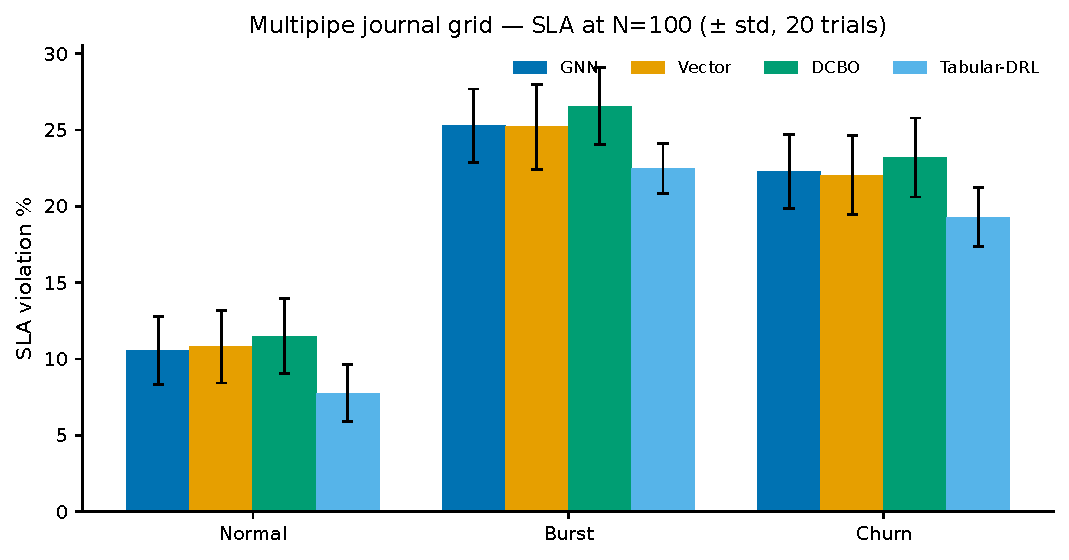
\includegraphics[width=0.82\linewidth]{fig06_sla_journal10.pdf}
\caption{Multipipe journal-grid SLA at $N{=}100$ (20 trials).}
\label{fig:j10}
\end{figure}
\FloatBarrier

\begin{figure}[htbp]
\centering

\includegraphics[width=0.82\linewidth]{fig11_holm.pdf}
\caption{Holm-adjusted $p$-values for paired SLA tests at $N{=}100$ (20 trials).}
\label{fig:holm}
\end{figure}
\FloatBarrier

\subsection{Tuning lock and offline path}
The 5-trial multipipe lock (Table~\ref{tab:champ}, Fig.~\ref{fig:champ}) fixed
offline weights and hyperparameters before the journal grid; we treat it as a
tuning lock, not the primary statistical claim. Without imported weights, an
earlier online-only medium put Vector slightly ahead of GraphSAGE while both beat
DCBO (Table~\ref{tab:online}), so the offline structure-weighted path is part
of the named GraphSAGE pipeline rather than a free online GNN-over-Vector gap.

\begin{table}[htbp]
\centering
\caption{Multipipe tuning lock: mean SLA \% (5 trials, $N{=}100$).}
\label{tab:champ}
\small
\begin{tabular}{@{}rllll@{}}
\toprule
$N$ & Scenario & Dyna-Bound (GS) & Dyna-Bound (V) & DCBO \\
\midrule
100 & Normal & \textbf{10.64} & 10.98 & 11.48 \\
100 & Burst & \textbf{24.89} & 25.35 & 26.13 \\
100 & Churn & \textbf{22.31} & 22.43 & 23.21 \\
\bottomrule
\end{tabular}
\end{table}

\begin{figure}[htbp]
\centering

\includegraphics[width=0.82\linewidth]{fig05_sla_champion.pdf}
\caption{Multipipe tuning-lock SLA at $N{=}100$ (5 trials).}
\label{fig:champ}
\end{figure}
\FloatBarrier

\begin{table}[htbp]
\centering
\caption{Earlier online-only multipipe medium (context; pre-lock).}
\label{tab:online}
\small
\begin{tabular}{@{}rllll@{}}
\toprule
$N$ & Scenario & Online DB (GS) & Dyna-Bound (V) & DCBO \\
\midrule
100 & Normal & 10.34 & \textbf{10.25} & 11.21 \\
100 & Burst & 24.39 & \textbf{24.09} & 26.42 \\
100 & Churn & 21.15 & \textbf{21.13} & 23.04 \\
\bottomrule
\end{tabular}
\end{table}

\subsection{Surveillance DAG}
Table~\ref{tab:surv} and Fig.~\ref{fig:surv} summarize the surveillance grid.
At $N{=}100$ the hybrid (Vector and GraphSAGE coincide on this shallow app) lowers
mean SLA against DCBO at matched overhead. At $N\in\{300,500\}$ the curves meet
because the blend gate hands ranking back to DCBO (Fig.~\ref{fig:scale}).

\begin{table}[htbp]
\centering
\caption{Surveillance DAG: mean SLA violation \% (5 trials).}
\label{tab:surv}
\small
\begin{tabular}{@{}rlll@{}}
\toprule
$N$ & Scenario & Hybrid & DCBO \\
\midrule
100 & Normal & \textbf{11.51} & 13.31 \\
100 & Burst & \textbf{14.02} & 14.78 \\
100 & Churn & \textbf{14.58} & 15.37 \\
300 & all & $\approx$0.48--0.51 & $\approx$0.48--0.50 \\
500 & all & $\approx$0.57--0.59 & $\approx$0.57--0.59 \\
\bottomrule
\end{tabular}
\end{table}

\begin{figure}[htbp]
\centering
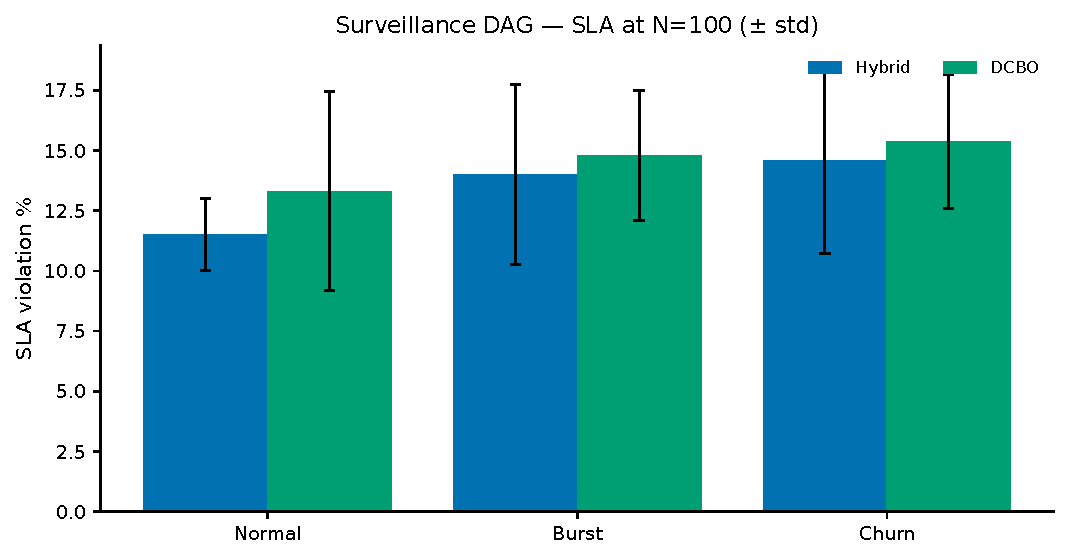
\includegraphics[width=0.82\linewidth]{fig04_sla_surveillance.pdf}
\caption{Surveillance SLA at $N{=}100$ (mean $\pm$ std, 5 trials).}
\label{fig:surv}
\end{figure}
\FloatBarrier

\subsection{Scale, overhead, and sensitivity}
Fig.~\ref{fig:scale} shows surveillance mean SLA versus target size.
Fig.~\ref{fig:oh} shows matched overhead for colony-plane hybrids and DCBO.
One-factor Burst sweeps (Fig.~\ref{fig:sens}) place $\beta{=}0.60$ and
$\varepsilon{=}0.02$ in the interior of mild SLA variation; deadline scale
shifts absolute SLA sharply (as expected) while hybrid-over-DCBO direction holds at
scales 8 and 12. The gate uses the live fog count ($n_f\ge 450\Rightarrow$
exact DCBO).

\begin{figure}[htbp]
\centering

\includegraphics[width=0.82\linewidth]{fig07_scalability.pdf}
\caption{Surveillance mean SLA versus target size $N$ (averaged over scenarios).}
\label{fig:scale}
\end{figure}

\begin{figure}[htbp]
\centering
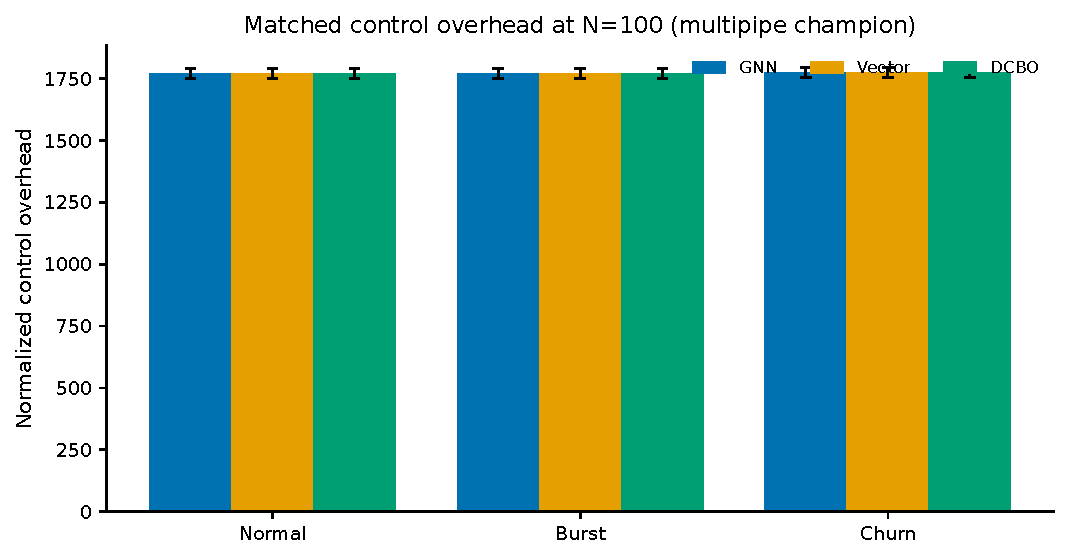
\includegraphics[width=0.82\linewidth]{fig08_overhead.pdf}
\caption{Normalized control overhead for colony-plane methods ($N{=}100$).
GraphSAGE, Vector, and DCBO remain matched.}
\label{fig:oh}
\end{figure}

\begin{figure}[htbp]
\centering
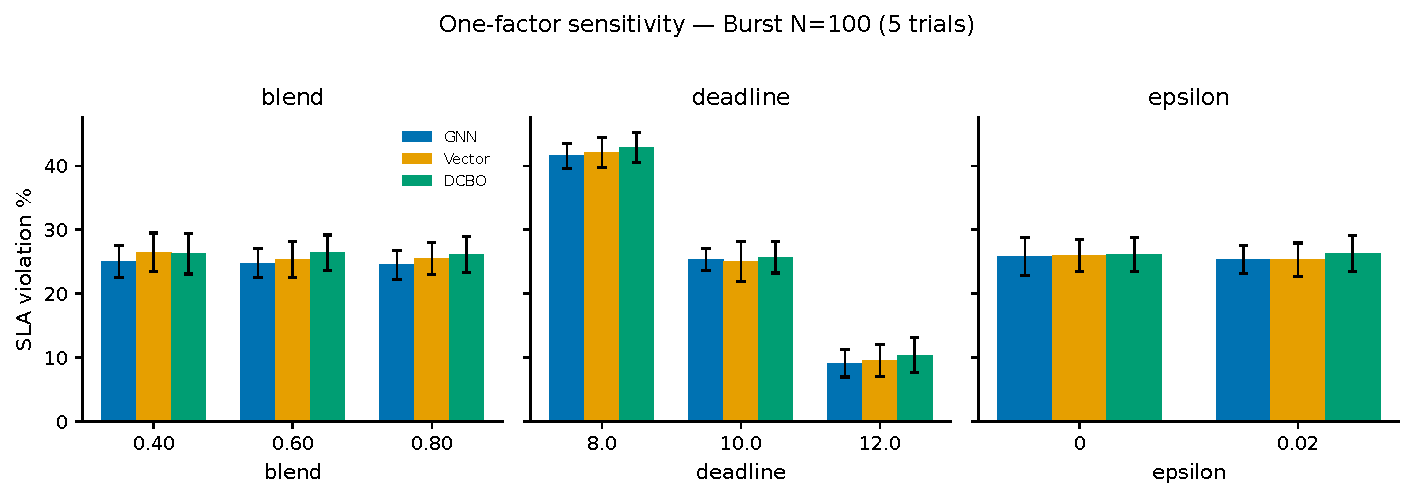
\includegraphics[width=0.95\linewidth]{fig13_sensitivity.pdf}
\caption{One-factor sensitivity on Burst $N{=}100$ (5 trials): blend, deadline
scale, and $\varepsilon$.}
\label{fig:sens}
\end{figure}
\FloatBarrier

\subsection{\texorpdfstring{Large-$N$ check}{Large-N check}}
At $N{=}1000$ (Table~\ref{tab:n1000}, Fig.~\ref{fig:n1000}) absolute SLA is low
and overhead matches ($\approx$2112--2140). Burst/churn means still favor GraphSAGE;
Holm tests after correction remain mostly non-significant, consistent with
near-parity under the large-$N$ blend gate.

\begin{table}[htbp]
\centering
\caption{Multipipe at $N{=}1000$: mean SLA \% (10 trials).}
\label{tab:n1000}
\small
\begin{tabular}{@{}llllr@{}}
\toprule
Scenario & Dyna-Bound (GS) & Dyna-Bound (V) & DCBO & Overhead \\
\midrule
Normal & 0.82 & \textbf{0.80} & 0.81 & 2112 \\
Burst & \textbf{2.53} & 3.13 & 3.59 & 2112 \\
Churn & \textbf{1.94} & 2.27 & 2.70 & 2140 \\
\bottomrule
\end{tabular}
\end{table}

\begin{figure}[htbp]
\centering
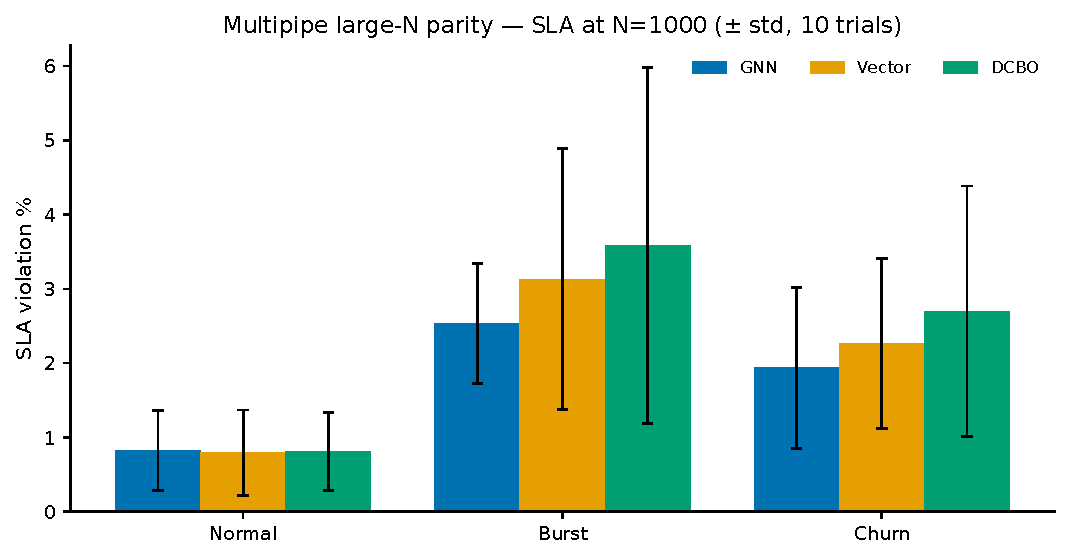
\includegraphics[width=0.78\linewidth]{fig09_sla_n1000.pdf}
\caption{Multipipe SLA at $N{=}1000$ (mean $\pm$ std, 10 trials).}
\label{fig:n1000}
\end{figure}
\FloatBarrier

\subsection{CRT-bounded DQN/PPO references and hard node failures}
Table~\ref{tab:dqnppo} is a separate five-trial multipipe lock that adds the
lightweight CRT-bounded DQN/PPO scorers. Means for GraphSAGE, Vector, and DCBO
need not match Table~\ref{tab:journal}: different trial counts and seeds, and
this table is only for colony-plane neural references, not for the Holm claim.
On this lock the hybrids again sit near or below DCBO; DQN and PPO are more
variable (larger std) and do not dominate the hybrid under the same CRT bound.

Hard fog-router failures at mid-run ($5\%$, $10\%$, $20\%$ of router nodes)
trigger an L3 reconcile. Table~\ref{tab:fail} reports SLA under that stress
together with how many hosts were taken down, how many mapped modules sat on
them, and the simulated time until the first post-failure reconcile. Host counts
and reconcile latency are largely properties of the shared control plane, so
they look similar across colony-plane methods; the useful comparison is the SLA
column in Table~\ref{tab:dqnppo}. Churn remains the membership scenario; failure
is a separate hard-down test.

\begin{table}[htbp]
\centering
\caption{CRT-bounded DQN/PPO vs hybrids and DCBO (multipipe, $N{=}100$,
5 trials; mean $\pm$ std SLA \%). Separate seed lock from Table~\ref{tab:journal}.}
\label{tab:dqnppo}
\small
\begin{tabular}{@{}llllll@{}}
\toprule
Scenario & GS & V & DCBO & DQN & PPO \\
\midrule
Normal & $9.96{\pm}1.48$ & $10.17{\pm}2.09$ & $11.33{\pm}2.69$ & $12.55{\pm}3.24$ & $13.03{\pm}4.46$ \\
Burst & $23.96{\pm}1.00$ & $23.86{\pm}1.41$ & $26.24{\pm}2.50$ & $23.36{\pm}5.43$ & $26.88{\pm}4.08$ \\
Churn & $21.47{\pm}1.61$ & $20.75{\pm}1.11$ & $23.13{\pm}2.37$ & $21.74{\pm}5.35$ & $24.15{\pm}4.25$ \\
Fail $5\%$ & $21.07{\pm}1.48$ & $20.10{\pm}1.10$ & $23.13{\pm}2.43$ & $22.00{\pm}5.06$ & $23.87{\pm}4.36$ \\
Fail $10\%$ & $21.00{\pm}1.26$ & $20.80{\pm}1.42$ & $23.45{\pm}3.28$ & $22.41{\pm}5.24$ & $24.06{\pm}4.53$ \\
Fail $20\%$ & $20.96{\pm}1.73$ & $21.19{\pm}1.34$ & $22.94{\pm}3.17$ & $22.33{\pm}4.96$ & $23.66{\pm}4.25$ \\
\bottomrule
\end{tabular}
\end{table}

\begin{table}[htbp]
\centering
\caption{Hard fog-router failures (multipipe, $N{=}100$, 5 trials): mean $\pm$ std
hosts taken down, modules that had been mapped onto them, and simulated ms to
the first post-failure reconcile (shared control-plane timing; compare SLA in
Table~\ref{tab:dqnppo}).}
\label{tab:fail}
\small
\begin{tabular}{@{}lllll@{}}
\toprule
Fail \% & Method & Hosts & Modules lost & Recovery (ms) \\
\midrule
5 & Dyna-Bound (GS) & $1.0{\pm}0.0$ & $4.8{\pm}3.0$ & $5.0{\pm}0.0$ \\
5 & Dyna-Bound (V) & $1.0{\pm}0.0$ & $4.8{\pm}3.0$ & $5.0{\pm}0.0$ \\
5 & DCBO & $1.0{\pm}0.0$ & $4.8{\pm}3.0$ & $5.0{\pm}0.0$ \\
5 & Colony-DQN & $1.0{\pm}0.0$ & $4.8{\pm}3.0$ & $5.0{\pm}0.0$ \\
5 & Colony-PPO & $1.0{\pm}0.0$ & $4.8{\pm}3.0$ & $5.0{\pm}0.0$ \\
10 & Dyna-Bound (GS) & $2.0{\pm}0.0$ & $8.4{\pm}4.1$ & $5.0{\pm}0.0$ \\
10 & Dyna-Bound (V) & $2.0{\pm}0.0$ & $8.4{\pm}4.1$ & $5.0{\pm}0.0$ \\
10 & DCBO & $2.0{\pm}0.0$ & $8.4{\pm}4.1$ & $5.0{\pm}0.0$ \\
10 & Colony-DQN & $2.0{\pm}0.0$ & $8.4{\pm}4.1$ & $5.0{\pm}0.0$ \\
10 & Colony-PPO & $2.0{\pm}0.0$ & $8.4{\pm}4.1$ & $5.0{\pm}0.0$ \\
20 & Dyna-Bound (GS) & $4.0{\pm}0.0$ & $16.8{\pm}1.8$ & $5.0{\pm}0.0$ \\
20 & Dyna-Bound (V) & $4.0{\pm}0.0$ & $16.8{\pm}1.8$ & $5.0{\pm}0.0$ \\
20 & DCBO & $4.0{\pm}0.0$ & $16.8{\pm}1.8$ & $5.0{\pm}0.0$ \\
20 & Colony-DQN & $4.0{\pm}0.0$ & $16.8{\pm}1.8$ & $5.0{\pm}0.0$ \\
20 & Colony-PPO & $4.0{\pm}0.0$ & $16.8{\pm}1.8$ & $5.0{\pm}0.0$ \\
\bottomrule
\end{tabular}
\end{table}

\subsection{Named baselines and Pareto view}
FogPlan, Greedy-Nearest, and Static-DCBO can post lower multipipe SLA than the
colony hybrids (Table~\ref{tab:base}, Fig.~\ref{fig:base}), but their overhead
and colony counts are not comparable. Fig.~\ref{fig:pareto} plots SLA against
normalized overhead on Burst: flat methods sit cheaper; colony-plane methods
cluster together; tabular DRL sits between them on cost while leading SLA inside
the cold-start view. We therefore defend a within-plane gain over DCBO at matched
hybrid/DCBO overhead, not a win over every flat placer.

\begin{table}[t]
\centering
\caption{Multipipe $N{=}100$: flat baselines (5 trials) beside the tuning-lock
colony means. Overhead is not matched across planes.}
\label{tab:base}
\scriptsize
\setlength{\tabcolsep}{2.5pt}
\resizebox{\columnwidth}{!}{%
\begin{tabular}{@{}lrrrrrr@{}}
\toprule
Scenario & FogPlan & Greedy & Static & DB (GS) & DB (V) & DCBO \\
\midrule
Normal & 8.28 & \textbf{7.32} & 9.25 & 10.64 & 10.98 & 11.48 \\
Burst & 23.24 & 22.63 & \textbf{21.61} & 24.89 & 25.35 & 26.13 \\
Churn & 19.88 & 19.37 & \textbf{19.02} & 22.31 & 22.43 & 23.21 \\
Overhead & 253 & 659 & 760 & $\approx$1769 & $\approx$1769 & $\approx$1769 \\
Colonies & 1 & 1 & 19 & $\approx$7.6 & $\approx$7.6 & $\approx$7.6 \\
\bottomrule
\end{tabular}%
}
\end{table}

\begin{figure}[htbp]
\centering
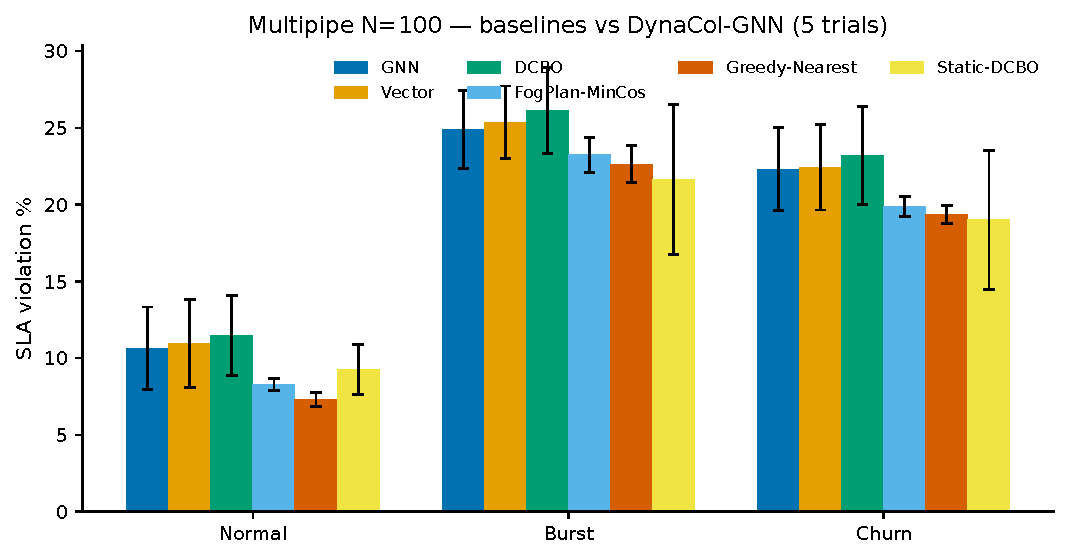
\includegraphics[width=0.88\linewidth]{fig10_baselines.pdf}
\caption{Flat baselines versus colony-bounded methods on multipipe $N{=}100$
(5 trials).}
\label{fig:base}
\end{figure}

\begin{figure}[htbp]
\centering

\includegraphics[width=0.78\linewidth]{fig12_pareto.pdf}
\caption{Pareto view: SLA vs normalized control overhead (Burst, $N{=}100$).}
\label{fig:pareto}
\end{figure}
\FloatBarrier

\subsection{Companion ablations}
\label{sec:ablations}

Table~\ref{tab:ablate} reports three 5-trial multipipe checks against the
bounded GraphSAGE smoke lock (same seeds/props except the stated factor).

\paragraph{CRT action-set ablation.}
Raising the L2 pool from CRT top-$K{=}5$ to a global fog top-$K{=}50$
(\texttt{crtAblate}) cuts mean SLA violation by roughly 4--5 points while the
reported CRT/GRT overhead stays matched. The bound is therefore a deliberate
visibility limit under decentralized tables. Giving the simulator a global
candidate list without charging discovery traffic shows how much SLA the CRT
withholds; the method keeps that limit to preserve bounded messaging.

\paragraph{Offline import.}
Removing imported GraphSAGE weights (online-only fine-tune from random init)
raises GraphSAGE SLA by about 0.7--1.8 points versus the locked import+FT path, so
the offline BC+ranking stage contributes measurable quality under the same
online hybrid.

\paragraph{$\beta{=}0$ delegation.}
Forcing $\beta{=}0$ routes L2 to exact DCBO; GraphSAGE and DCBO means stay within a
fraction of a point, confirming the scale-aware hand-back path.

\begin{table}[htbp]
\centering
\caption{Companion ablations (multipipe, $N{=}100$, 5 trials): mean SLA \%.
Bounded GraphSAGE is the $n{=}5$ smoke lock; CRT-ablate expands L2 to global top-50.}
\label{tab:ablate}
\scriptsize
\begin{tabular}{@{}llll@{}}
\toprule
Scenario & Bounded DB (GS) & CRT-ablate DB (GS) & No-offline DB (GS) \\
\midrule
Normal & 10.32 & \textbf{5.46} & 11.38 \\
Burst & 24.88 & \textbf{20.93} & 26.68 \\
Churn & 22.39 & \textbf{17.24} & 23.05 \\
\bottomrule
\end{tabular}
\end{table}

\section{Discussion}
\label{sec:disc}

The question this paper answers is narrow: once CRT/GRT traffic is fixed by
DynaCol, does hybrid L2 ranking beat plain DCBO? On the $n{=}20$ multipipe grid
the answer is yes (Table~\ref{tab:journal}). Paired gaps survive Holm correction,
with Cohen's $d$ for GraphSAGE$-$DCBO about $0.61$--$1.14$
\cite{cohen_power1988}. The effect is medium in the statistical sense and small
on the absolute SLA axis (roughly one percentage point). That is still useful
in this setting because the gain does not buy extra control messages: the
hybrids and DCBO share the same overhead band near $1770$ normalized units.
Formation, FCM handover, and table size limits remain DynaCol's; only the L2
score changes.

GraphSAGE and the vector scorer finish essentially tied on that grid. We keep
GraphSAGE as the structured default because it carries CRT affinity edges and
an offline import path
\cite{hamilton_graphsage2017,xu_gin_iclr2019,ross_aistats2011_dagger}, but the
hybrid-versus-DCBO gap does not depend on message passing for these shallow
CRT neighborhoods. Calling the method ``colony-bounded hybrid learning'' is
therefore more accurate than selling it as a GNN win.

Tabular $\varepsilon$-greedy DRL often records the lowest SLA means in the
colony view, sometimes with slightly less overhead. We do not hide that. The
submitted design is still the hybrid for three practical reasons. First, it
stays anchored to DCBO, so when the live fog count crosses the large-$N$ gate
ranking falls back to the same deterministic rule operators already trust.
Second, the offline BC+ranking import gives GraphSAGE a warm start that the
tabular learner does not use. Third, the hybrid is built to keep CRT/GRT
overhead matched to DCBO by construction; the tabular policy is a useful
reference, not a drop-in replacement for that contract. Against open-set
GNN-RL placers that score much wider device sets
\cite{lera_jsup2024_gnn,chen_tmc2024_dgddpg} we make no ranking claim.

The CRT ablation (Table~\ref{tab:ablate}) is easy to misread. Opening L2 to a
global fog top-$50$ without charging discovery traffic lowers SLA violation by
several points. That shows how much QoS the colony bound withholds; it does not
show that a larger table is ``free.'' A fairer follow-up would bill inventory
messages. Setting $\beta{=}0$ recovers DCBO within a fraction of a point, which
checks the hand-back path. Removing offline weights hurts GraphSAGE by about
$0.7$--$1.8$ points under the same online hybrid.

Several grids appear in the paper on purpose. The Holm claim uses only
Table~\ref{tab:journal}. Table~\ref{tab:dqnppo} is a later five-trial lock for
lightweight CRT-bounded DQN/PPO references; means for the shared methods can
drift with seeds and should not be mixed into the $n{=}20$ tests. On that lock
DQN/PPO do not overturn the hybrid, and their trial-to-trial spread is larger.
They are small shared-MLP scorers with one-step updates, not full open-host
deep RL systems.

Flat baselines in Table~\ref{tab:base} and Fig.~\ref{fig:pareto} answer a
different question: what SLA is possible if one ignores cold-start colony cost.
FogPlan and related methods can look better on raw SLA while spending far less
(or structuring the fabric differently). That comparison is informative and
intentionally unmatched.

\paragraph{Limits.}
\label{sec:limits}
Evidence is simulation-only (iFogSim2); we have not run a physical testbed.
Deadlines on multipipe are scaled (Fig.~\ref{fig:sens}), so absolute SLA levels
are workload-specific even when method order is stable. Offline weights come
from logged trajectories rather than a fully on-policy loop
\cite{levine_offline_rl2020}. The CRT-ablate experiment still omits discovery
cost. Edgeward was dropped on multipipe for runtime. DynaCol itself is cited as
an unpublished companion; Appendix~\ref{app:dynacol} reprints the reused
algorithms, and the public repository carries the shared runtime. Hard router
failures at $5$--$20\%$ are reported, but reconcile latency is mostly a
control-plane timer shared across colony methods. We did not build an open-set
DQN/PPO, a centralized Oracle at large $N$, or an energy-primary objective;
energy is exported by the simulator yet is not the headline metric here.
Control messages may carry service and host identifiers; securing them
(authentication, encryption) is outside this study. Encoder decisions remain
only partly readable through the DCBO term.

\paragraph{Offline cost.}
GraphSAGE may load a HID$=$16 JSON weight file and fine-tune online. That
offline pass is separate from the per-decision CRT/GRT overhead in the tables;
its wall-clock cost scales with the log, not with $N$ at inference time.

\section{Conclusion}
\label{sec:conc}

Dyna-Bound ranks fog hosts inside cold-start colony tables: L2 mixes a small
online scorer with DCBO, actions stay in CRT/GRT top-$K$, and large fabrics
return to exact DCBO. On iFogSim2 multipipe workloads at $N{=}100$ the hybrid
beats DCBO at matched overhead, with paired Holm-significant gaps at $n{=}20$
and medium effect sizes; the absolute SLA change is modest. GraphSAGE and the
vector scorer are statistically tied, so the result is about bounded hybrid
ranking. Tabular $\varepsilon$-greedy learning can lead raw SLA inside the same
view and is kept as a reference; the hybrid is submitted for its DCBO anchor,
large-$N$ hand-back, and overhead contract. CRT ablations show how much QoS the
bound withholds; offline import helps the GraphSAGE path; $\beta{=}0$ recovers
DCBO. Flat baselines and node-failure trials round out the picture without
changing that within-plane claim.

Natural next steps are to bill discovery traffic when the action set grows,
tighten offline training toward on-policy data, and move selected scenarios onto
a testbed.

\section*{Declarations}

\paragraph{Funding.}
The authors declare that no funds, grants, or other support were received
during the preparation of this manuscript.

\paragraph{Competing interests.}
The authors have no relevant financial or non-financial interests to disclose.

\paragraph{Author contributions.}
R.N.\ designed the method, implemented the experiments, and drafted the
manuscript. A.G.\ supervised the research and revised the manuscript. Both
authors read and approved the final manuscript.

\paragraph{Editorial tools.}
The authors used AI-assisted editing tools for language polishing, bibliography
formatting, and LaTeX layout checks. All scientific claims, experimental
designs, numerical results, and final wording were reviewed and approved by the
authors.

\paragraph{Data availability.}
Simulation configs, trial CSVs, summary tables, and figure scripts are in the
public JoS artifact repository
\url{https://github.com/RouhollahNabati/Dyna-Bound}
(\texttt{configs/}, \texttt{evaluation/results/}, \texttt{evaluation/}).
The parent DynaCol / iFogSim2 runtime remains separately available at
\url{https://github.com/RouhollahNabati/DynaCol}.

\paragraph{Code availability.}
Dyna-Bound source is available at
\url{https://github.com/RouhollahNabati/Dyna-Bound}
(Java under \texttt{ifogsim2/src/org/fog/dynacolgnn/}; Python tools and grids
at the repository root). The unchanged DynaCol control-plane code stays in
\url{https://github.com/RouhollahNabati/DynaCol}.

\appendix
\section{Reused DynaCol algorithms}
\label{app:dynacol}

For self-containment relative to the prior DynaCol manuscript
\cite{nabati_dynacol_cluster2026}, we reprint the cold-start, handover, and
DCBO L1--L3 skeletons that this paper leaves unchanged. These algorithms are
\emph{not} claimed as contributions here.

\begin{algorithm}[t]
\caption{Cold-start join (Create\_And\_Add\_FogNode)}
\label{alg:cold}
\begin{algorithmic}[1]
\Require join event for node $FID$; timers $W_t$, $T_{\mathrm{adv}}$; radius MaxColonySize
\State state $\leftarrow$ Unassigned
\State broadcast QueryColony($FID$); start timer $T$
\If{no response and $T\ge W_t$}
  \State self-elect FCM; init CRT/GRT; AdvertisePeriodically($T_{\mathrm{adv}}$)
\Else
  \State $resp\leftarrow$ best JoinScore response
  \If{$L(FID,resp.\mathrm{FCM})<$ MaxColonySize}
    \State JoinOrNegotiate($resp$) \Comment{Alg.~\ref{alg:handover}}
  \EndIf
\EndIf
\end{algorithmic}
\end{algorithm}

\begin{algorithm}[t]
\caption{JoinOrNegotiate (potency-based FCM handover)}
\label{alg:handover}
\begin{algorithmic}[1]
\Require response $resp$ with colony id, FCM, CRT
\If{self is FCM-candidate and Potency(self)$>$Potency($resp$.FCM)$+\varepsilon$ and cooldown elapsed}
  \State negotiate ManagerTakeoverRequest; on accept promote self and merge CRT
\Else
  \State join $resp$.ColonyID under $resp$.FCM; FCM updates CRT/GRT
\EndIf
\end{algorithmic}
\end{algorithm}

\begin{algorithm}[t]
\caption{DCBO\_PlaceService (L1--L3)}
\label{alg:dcbo}
\begin{algorithmic}[1]
\Require service $s$, current host $h_{\mathrm{cur}}$, tables CRT, GRT
\If{$h_{\mathrm{cur}}$ feasible and SLA-safe}
  \State \Return $h_{\mathrm{cur}}$ \Comment{L1 sticky}
\EndIf
\State Cand $\leftarrow$ top-$K_{\mathrm{crt}}$ feasible CRT hosts by $J(s,\cdot)$
\If{Cand $\ne\emptyset$}
  \State \Return $\arg\min$ Cand \Comment{L2 local}
\EndIf
\For{all col in top-$K_{\mathrm{grt}}$(GRT)}
  \If{DelegatePlace($s$, col.FCM) succeeds}
    \State \Return delegated host \Comment{L2 neighbor}
  \EndIf
\EndFor
\State \Return cloud by latency/cost \Comment{L3}
\end{algorithmic}
\end{algorithm}

\section{Hyperparameters}
\begin{table}[h]
\centering
\caption{Locked-grid hyperparameters.}
\label{tab:hyper}
\small
\begin{tabular}{@{}ll@{}}
\toprule
Parameter & Default / note \\
\midrule
CRT top-$K_{\mathrm{crt}}$ / GRT top-$K_{\mathrm{grt}}$ & $5$ / $3$ \\
$\varepsilon$ (hybrid) & $0.02$ on multipipe ($0$ at large $N$) \\
$\varepsilon$ (tabular DRL) & $0.15$ \\
Vector / GraphSAGE LR & $0.05$ / $0.04$ \\
GraphSAGE hidden & $16$, 2 layers, $\tanh$ \\
Host / context dims & $8$ / $8$ \\
Blend (multipipe) & $0.60$ \\
Multipipe SLA scale & $10.0$ \\
Large-$N$ gate & $n_f\ge 450$ $\rightarrow$ exact DCBO \\
Offline objective & reward-advantage BC + structure ranking \\
Trials & 5 (tuning lock/baselines); 20 (journal $N{=}100$); 10 ($N{=}1000$) \\
\bottomrule
\end{tabular}
\end{table}
\FloatBarrier

\bibliographystyle{apalike}
\bibliography{refs}

\end{document}
